\documentclass[11pt]{article}
\usepackage{amsmath, amssymb, amsthm}
\usepackage{geometry}
\usepackage{hyperref}
\usepackage{tikz}
\usetikzlibrary{arrows.meta, positioning}
\geometry{margin=1in}

\title{Notes 00 \\ Review of Statistics: \\ Statistical Inference}
\author{DATA 000: Advanced Computational Methods in Education and the Social Sciences}
\date{Alexander \\ Spring 2026}

\begin{document}

\maketitle

\tableofcontents

\section{Introduction}

\textbf{Statistical inference} is the process of using data from a sample to draw conclusions about a population. Inference is the foundation of quantitative research in education and the social sciences, enabling us to estimate unknown parameters, test hypotheses, and generalize findings beyond the observed data\ [6][7][8].

\section{Key Concepts}

\subsection{Population, Sample, Parameter, Statistic}

\begin{itemize}
    \item \textbf{Population:} The entire group of interest (e.g., all students in a district).
    \item \textbf{Sample:} A subset of the population, selected for analysis.
    \item \textbf{Parameter:} A numerical summary of the population (e.g., population mean $\mu$).
    \item \textbf{Statistic:} A numerical summary computed from the sample (e.g., sample mean $\bar{x}$).
\end{itemize}

\subsection*{Visualization: Population vs. Sample}
\begin{center}
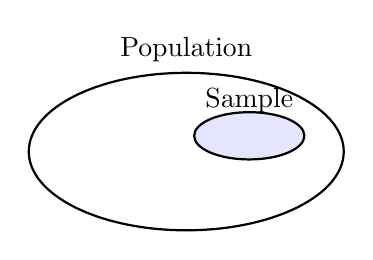
\begin{tikzpicture}[scale=1]
  % Population ellipse
  \draw[thick] (0,0) ellipse (2 and 1);
  \node at (0,1.3) {Population};
  % Sample ellipse
  \draw[thick, fill=blue!10] (0.8,0.2) ellipse (0.7 and 0.3);
  \node at (0.8,0.65) {Sample};
\end{tikzpicture}
\end{center}

\section{Sampling Distributions}

A \textbf{sampling distribution} is the probability distribution of a statistic over all possible samples from the population.

\textbf{Example:} The distribution of sample means ($\bar{x}$) from repeated samples.

\subsection*{Visualization: Sampling Distribution of the Mean}
\begin{center}
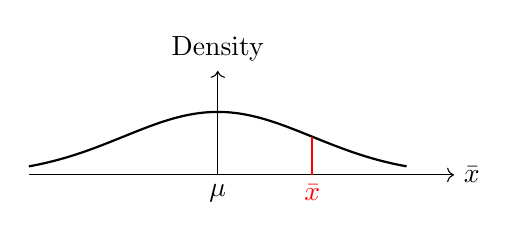
\begin{tikzpicture}[scale=1.2]
  % X-axis
  \draw[->] (-2,0) -- (2.5,0) node[right] {$\bar{x}$};
  % Y-axis
  \draw[->] (0,0) -- (0,1.1) node[above] {Density};
  % Normal curve
  \draw[thick, domain=-2:2, samples=100] plot (\x, {exp(-\x*\x/2)/1.5});
  % Mean
  \draw[dashed] (0,0) -- (0,0.7);
  \node[below] at (0,0) {$\mu$};
  % Example sample mean
  \draw[red, thick] (1,0) -- (1,0.4);
  \node[below, red] at (1,0) {$\bar{x}$};
\end{tikzpicture}
\end{center}

\section{Estimation}

\subsection{Point Estimation}

A \textbf{point estimate} is a single value used to estimate a population parameter.

\textbf{Example:} $\bar{x}$ estimates $\mu$; $s^2$ estimates $\sigma^2$.

\subsection{Interval Estimation (Confidence Intervals)}

A \textbf{confidence interval} gives a range of plausible values for a parameter, based on sample data.

\[
\text{CI for } \mu: \quad \bar{x} \pm z^* \frac{\sigma}{\sqrt{n}}
\]
If $\sigma$ unknown, use $t^*$ and $s$.

\textbf{Interpretation:} If we repeat the sampling many times, about 95\% of calculated intervals will contain the true parameter.

\subsection*{Example: Confidence Interval (Education, with Solution)}

A random sample of $n=36$ students has mean test score $\bar{x}=78$, sample standard deviation $s=12$. Find a 95\% confidence interval for the population mean.

\textbf{Solution:}

\[
\text{SE} = \frac{12}{\sqrt{36}} = 2
\]
\[
t^* \approx 2.03 \text{ (for } df=35)
\]
\[
\text{CI: } 78 \pm 2.03 \times 2 = 78 \pm 4.06 = [73.94, 82.06]
\]

\textbf{Interpretation:} We are 95\% confident the true mean lies between 73.94 and 82.06.

\section{Hypothesis Testing}

\subsection{Logic and Steps}

\begin{enumerate}
    \item \textbf{State the hypotheses:}
        \begin{itemize}
            \item $H_0$: null hypothesis (no effect or difference)
            \item $H_A$: alternative hypothesis (effect or difference exists)
        \end{itemize}
    \item \textbf{Choose significance level} ($\alpha$, commonly 0.05)
    \item \textbf{Compute test statistic} (e.g., $z$, $t$, $F$, $\chi^2$)
    \item \textbf{Find p-value} or compare to critical value
    \item \textbf{Draw a conclusion}: Reject or do not reject $H_0$
\end{enumerate}

\subsection{Types of Errors}

\begin{itemize}
    \item \textbf{Type I error}: Rejecting $H_0$ when it is true (false positive). Probability = $\alpha$.
    \item \textbf{Type II error}: Not rejecting $H_0$ when $H_A$ is true (false negative). Probability = $\beta$.
    \item \textbf{Power}: Probability of correctly rejecting $H_0$ ($1-\beta$).
\end{itemize}

\subsection*{Visualization: Hypothesis Test Decision}
\begin{center}
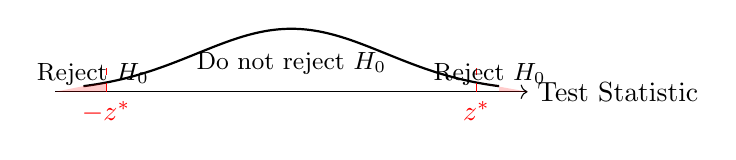
\begin{tikzpicture}[scale=1.2]
  % X-axis
  \draw[->] (-2.5,0) -- (2.5,0) node[right] {Test Statistic};
  % Normal curve
  \draw[thick, domain=-2.2:2.2, samples=100] plot (\x, {exp(-\x*\x/2)/1.5});
  % Critical values
  \draw[dashed, red] (1.96,0) -- (1.96,0.25);
  \draw[dashed, red] (-1.96,0) -- (-1.96,0.25);
  \node[below, red] at (1.96,0) {$z^*$};
  \node[below, red] at (-1.96,0) {$-z^*$};
  % Shade rejection regions
  \fill[red, opacity=0.2] (2.5,0) -- plot[domain=1.96:2.2] (\x, {exp(-\x*\x/2)/1.5}) -- (2.2,0) -- cycle;
  \fill[red, opacity=0.2] (-2.5,0) -- plot[domain=-2.2:-1.96] (\x, {exp(-\x*\x/2)/1.5}) -- (-1.96,0) -- cycle;
  \node at (2.1,0.18) {\small Reject $H_0$};
  \node at (-2.1,0.18) {\small Reject $H_0$};
  \node at (0,0.3) {\small Do not reject $H_0$};
\end{tikzpicture}
\end{center}

\section{Example: Hypothesis Test (Social Science, with Solution)}

A researcher wants to know if a new policy increased average weekly study hours for students. Before the policy, the mean was 10 hours. After, a sample of $n=25$ students had $\bar{x}=11.5$, $s=4$.

\textbf{Step 1:} $H_0: \mu=10$, $H_A: \mu>10$ (one-sided test).

\textbf{Step 2:} $\alpha=0.05$, $t^* \approx 1.71$ ($df=24$).

\textbf{Step 3:} $t = \frac{11.5-10}{4/\sqrt{25}} = \frac{1.5}{0.8} = 1.875$

\textbf{Step 4:} $1.875 > 1.71$, so reject $H_0$.

\textbf{Interpretation:} There is evidence the policy increased study hours.

\section{Multiple Comparisons and p-values}

When performing multiple hypothesis tests, the chance of a Type I error increases. Adjustments (e.g., Bonferroni correction) are used to control the overall error rate.

\section{Common Mistakes and Good Practices}

\begin{itemize}
    \item Confusing statistical significance with practical importance.
    \item Ignoring assumptions (e.g., normality, independence).
    \item Selective reporting (publication bias).
    \item Not reporting effect sizes or confidence intervals.
    \item Good practice: transparency, reproducibility, clear reporting.
\end{itemize}

\section{Summary Table: Key Elements of Inference}

\begin{tabular}{|l|l|}
\hline
\textbf{Concept} & \textbf{Description} \\
\hline
Parameter & Numerical summary of a population (e.g., $\mu$, $p$) \\
Statistic & Computed from sample data (e.g., $\bar{x}$, $\hat{p}$) \\
Point Estimate & Single value estimate for parameter \\
Confidence Interval & Range of plausible values for parameter \\
Hypothesis Test & Procedure to assess evidence against $H_0$ \\
p-value & Probability of observed (or more extreme) data if $H_0$ true \\
Type I Error & Rejecting $H_0$ when true ($\alpha$) \\
Type II Error & Not rejecting $H_0$ when false ($\beta$) \\
Power & $1-\beta$; probability of correctly rejecting $H_0$ \\
\hline
\end{tabular}

\section{Further Notes}

\begin{itemize}
    \item Statistical inference is central to research in education and social sciences\ [1][2][3][5][6].
    \item Both estimation and hypothesis testing are fundamental tools\ [6][8].
    \item Understanding the logic and limitations of inference is essential for critical data analysis and responsible research\ [7].
\end{itemize}

\end{document}
